\documentclass{beamer}
\usetheme{Madrid}
\usepackage{listings}
\usepackage{graphicx}
\usepackage{minted}
\usepackage{amsmath, amsthm}

\newtheorem{thm}{Theomème}
\newtheorem{pf}{Preuve}
\newtheorem{rmk}{Remarque}
\newtheorem{prp}{Proposition}
\newtheorem{df}{Définition}
\newtheorem{crll}{Corollaire}

\title{
    Sous groupes de $\mathbb{Z}/n \mathbb{Z} \times \mathbb{Z}/n\mathbb{Z}$
}
\subtitle{Projet Mathématiques-Informatique}
\institute[U. Paris Cité]{Université Paris Cité}
\author[Kevin G., Charly M.A.]{
    Kevin Garnier \\    Charly Martin-Avila
}
\date{\today}

\begin{document}

\begin{frame}
\titlepage
\end{frame}

\tableofcontents


\section{Quelques simplifications du problème}
\begin{frame}
\frametitle{Quelques simplifications du problème}
\tableofcontents[currentsection]
\end{frame}


\subsection{Décomposition de n en éléments irréductibles}
\begin{frame}
    \frametitle{Décomposition de n en éléments irréductibles}
    \begin{prp}
        Soit $n = \prod\limits_{i = 1}^k p_i^{\alpha_i}$ avec $p_i$ des nombres premiers distincts. Alors,
    
        \begin{align*}
            (\mathbb{Z}/n\mathbb{Z} \times \mathbb{Z}/n\mathbb{Z})
            \cong
            \prod\limits_{i = 1}^k (\mathbb{Z}/p_i^{\alpha_i}\mathbb{Z})^{2}
        \end{align*}
    \end{prp}
\end{frame}


\begin{frame}[fragile]
    \frametitle{Décomposition de n en éléments irréductibles}
    \begin{minted}{OCaml}
fonction rho_pollard P n x y k i d
    Si d <> 1:
        Retourne d
    Sinon :
        x = P ( x ) mod n
        d = pgcd (| y - x | , n )
        Si i = k :
            Retourne rho_pollard P n x x 2k (i+1) d
        Sinon 
            Retourne rho_pollard P n x y k (i+1) d
    \end{minted}
\end{frame}

\subsection{Simplification des sous-groupes}
\begin{frame}
\frametitle{Simplification des sous-groupes}
\begin{prp}<1->
    \center $\mathbb{Z}^2/n\mathbb{Z} \times n\mathbb{Z} \cong  \mathbb{Z}/n\mathbb{Z} \times \mathbb{Z}/n\mathbb{Z}$
\end{prp}
\begin{rmk}<2->
    Le problème se résout à trouver les sous-groupes $\mathbb{G}$ de $\mathbb{Z}$^2 tels que
    \begin{align*}
        H = \begin{pmatrix}
            a & c \\
            b & d \\
        \end{pmatrix}
    \end{align*}
    \center et
    \begin{align*}
        n\mathbb{Z} \times n\mathbb{Z} \subseteq \mathbb{G} = < 
            \begin{pmatrix}
                \overline{a} \\
                \overline{b}
            \end{pmatrix}
            ,
            \begin{pmatrix}
                \overline{c} \\
                \overline{d}
            \end{pmatrix}
            >
    \end{align*}
\end{rmk}
\end{frame}


\section{Matrices à coefficients entier et forme normales de Hermite}
\begin{frame}
\frametitle{Table des matières}
\tableofcontents[currentsection]
\end{frame}


\subsection{Matrices à coefficients entier}
\begin{frame}
\frametitle{Matrices à coefficients entier}

\begin{prp}
    Soient $A$ \in $\mathbb{M}_{m,n}(\mathbb{Z})$ et $Q$ \in $\mathbb{GL}_{n}(\mathbb{Z})$ alors
    \begin{align*}
        \mathrm{Im}(AQ) = \mathrm{Im}(A)
    \end{align*}
\end{prp}
\end{frame}


\subsection{Formes normales de Hermite}
\begin{frame}
\frametitle{Formes normales de Hermite}
\begin{df}
    Soit $A$ \in $\mathbb{M}_{m,n}(\mathbb{Z})$ alors, il existe une unique matrice échelonnée réduite suivant les colonnes $H$ \in $\mathbb{M}_{m,n}(\mathbb{Z})$ telle qu'il existe $Q$ \in  $\mathbb{GL}_{n}(\mathbb{Z})$ avec $H$ = $AQ$. La matrice $H$ s'appelle la forme normale de Hermite de $A$.
\end{df}
\end{frame}


\section{Génération et énumération des sous-groupes}
\begin{frame}
\frametitle{Table des matières}
\tableofcontents[currentsection]
\end{frame}


\subsection{Génération des sous-groupes}
\begin{frame}
\frametitle{Génération des sous-groupes}
\begin{itemize}
    \item Dans cette section, nous supposerons que $n$ = ${p}^{m}$
\end{itemize}
\begin{thm}
    Les seules matrices dont les colonnes génèrent un sous-groupe de $\mathbb{Z}/p^m\mathbb{Z} \times \mathbb{Z}/p^m\mathbb{Z}$ sont les matrices de la forme
    \begin{align*}
        H = \begin{pmatrix}
        p^a & 0 \\
        j & p^b 
        \end{pmatrix}
        \quad \text{avec } a \leq m, b \leq m \text{ et } j < p^b    
    \end{align*}\\
    \center ou
    \begin{align*}
        H = \begin{pmatrix}
        p^a & 0 \\
        jp^k & p^b 
        \end{pmatrix}
        \quad \text{avec } a \leq m, b \leq m, k \leq m \text{ et } j < p^(b-k)
    \end{align*}
\end{thm}
\end{frame}


\begin{frame}
\begin{crll}
    Soit la suite $(A_k)_{0 \leq k \leq n}$ telle que
    \begin{align*}
        A_0 = \{(a, b) \mid a + b \leq m \}
    \end{align*}
    \begin{align*}
        A_k = \{(a, b) \mid a \leq m, b \leq m, a + b = m + k \}  
    \end{align*}
    Alors, l’ensemble des matrices du théorème, c’est-à-dire, les matrices dont les colonnes
génèrent les sous-groupes $\mathbb{Z²}/p^m\mathbb{Z} \times p^m\mathbb{Z}$ est
    \begin{align*}
        M = \bigcup_{k=0}^{m} M_k
    \end{align*}
    \center où
    \begin{align*}
        M_k = \{ 
            \begin{pmatrix}
                p^a & 0 \\
                jp^k & p^b 
            \end{pmatrix}
            \mid (a, b) \in A_k, 0 \leq j \leq p^{(b-k)}
        \}
    \end{align*}
\end{crll}
\end{frame}


\subsection{Énumération des sous-groupes}
\begin{frame}
\frametitle{Énumération des sous-groupes}
\begin{thm}
    Soit $\psi: \mathbb{N}^2 \rightarrow \mathbb{N}$ définie par
    \begin{align*}
    \psi(p, n) = \sum_{i=0}^{n} (n - i)p^i + \sum_{i=0}^{n} \frac{1 - p^{n-i+1}}{1 - p}
    \end{align*}
    Alors, le nombre de sous groupe de $\mathbb{Z}/p^m\mathbb{Z} \times \mathbb{Z}/p^m\mathbb{Z}$ est $\psi(p,m)$
\end{thm}    
\end{frame}


\begin{frame}
\begin{prp}
    Soit n = \prod\limits_{i = 1}^k p_i^{\alpha_i} avec $p_i$ des nombres premiers distincts. Le nombre total de sous-groupes de $\mathbb{Z}/n\mathbb{Z} \times \mathbb{Z}/n\mathbb{Z}$ est
    \begin{align*}
    \prod_{i = 1}^{k} \psi(p_i,\alpha_i)
    = \prod_{i=1}^k\left(\sum_{j=0}^{\alpha_i}(\alpha_i-j)p_i^j +%
    \sum_{j = 0}^{\alpha_i}\frac{1- p_i^{\alpha_i-j+1}}{1 - p_i}\right)
    \end{align*}
\end{prp}
\end{frame}


\section{Génération du treillis}
\begin{frame}
\frametitle{Génération du treillis}
\tableofcontents[currentsection]
\end{frame}

\begin{frame}[fragile]
\frametitle{Génération du treillis}
\begin{minted}{OCaml}
fonction creer_treillis (G T) =
    G <- Trier G par la cardinalité
    L = Vide
    Pour chaque u dans G:
        Pour chaque v dans T[u]:
            Si not-exists (u, v0) dans L tel que v0  v
                Alors L $\cup$ {(u, v)}
    Retourner (G, L)
\end{minted}
\end{frame}


\section{Quelques résultats}
\begin{frame}
\frametitle{Table des matières}
\tableofcontents[currentsection]
\end{frame}


\subsection{Pour n = 2}
\begin{frame}
\frametitle{Pour n = 2}
\begin{itemize}
    \item Nombre de sous-groupe de $\mathbb{Z}/2\mathbb{Z} \times \mathbb{Z}/2\mathbb{Z}$ : 5
\end{itemize}
\begin{figure}
  \centering
  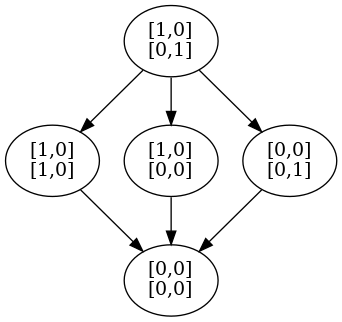
\includegraphics[width=0.5\textwidth]{Z2ZxZ2Z.png}
\end{figure}
\end{frame}


\subsection{Quelques valeur de la suite du nombre de sous-groupes}
\begin{frame}
\frametitle{Quelques valeur de la suite du nombre de sous-groupes}
\begin{center}
    \begin{tabular}{|c|c|c|c|c|c|c|c|c|c|c|c|}
        \hline
        n       & 0     & 1 & 2 & 3 & 4  & 5 & 6  & 7  & 8  & 9  & 10 \tabularnewline
        \hline
        $|\mathbb{Z}/n\mathbb{Z} \times \mathbb{Z}/n\mathbb{Z}|$ & $\infty$ & 1 & 5 & 6 & 15 & 8 & 30 & 10 & 37 & 23 & 40 \tabularnewline
        \hline
    \end{tabular}
\end{center}
\end{frame}


\section{Bibliographie}
\begin{frame}
\frametitle{Table des matières}
\tableofcontents[currentsection]
\end{frame}


\begin{frame}
\frametitle{Bibliographie}
\begin{itemize}
    \item COSTE Michel ; Algèbre linéaire sur les entiers ; Mars 2018
    \item Thomas H. Cormen, Charles Leiserson, Ronald Rivest, Clifford Stein ; Algorithmique : cours avec 957 exercices et 158 problèmes, 3e édition, Paris : Dunod ; DL 2010
    \item PERNET Clément ; Calcul de formes normales matricielles : de l’algorithmique à la mise en pratique ; Séminaire SIESTE ; ENS-Lyon ; 12 février 2013
    \item BERHURY Grégory ; Algèbre le grand combat : Cours et exercices ; 2e édition ; Paris : Calvage & Mounet ; 2020. 1215 p. (Mathématiques en devenir)
    \item Mario Hampejs, Nicki Holighaus, László Tóth, Christoph Wiesmeyr ; Representing and counting the subgroups of the group Zm × Zn ; 2012
\end{itemize}
\end{frame}


\end{document}
